\documentclass{beamer}
\usepackage{graphicx}
\usepackage{subcaption}
\title{Project WIT: Pear}
\author{Mattias Billast, Alexander Boucquey}
\date{\today}

\begin{document}

\begin{frame}
\frametitle{Overzicht project}
\tableofcontents
\end{frame}

\begin{frame}
\frametitle{Werkwijze}
\begin{enumerate}
\item Handgeschreven oplossing;
\item Uitwerken in matlab en verbeteren indien niet realistisch of correct (vergelijken met analytische oplossing);
\item Uitschrijven in c++;
\item Optimaliseren in c++.
\end{enumerate}
\end{frame}

\begin{frame}
\frametitle{Resultaten: Optimal CA}

\begin{columns}
\begin{column}{0.48\textwidth}
\begin{figure}
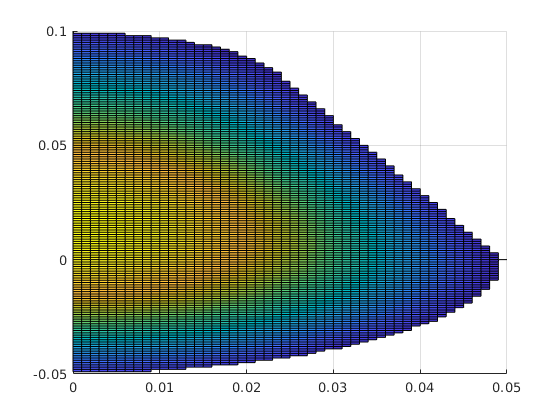
\includegraphics[width = 1\textwidth]{Optimal_CA_pear_CO2_boven.png}
\caption{CO2 voor Optimal CA.}
\end{figure}
\end{column}
	
\begin{column}{0.48\textwidth}
\begin{figure}
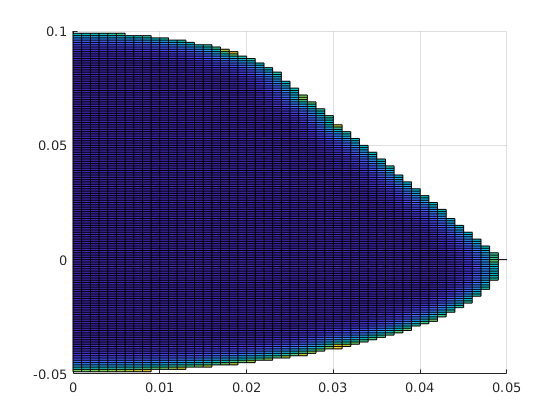
\includegraphics[width = 1\textwidth]{Optimal_CA_pear_O2_boven.png}
\caption{O2 voor Optimal CA.}
\end{figure}
\end{column}
\end{columns}


\end{frame}

\begin{frame}
\frametitle{Resultaten: Disorder inducing}
\begin{columns}
\begin{column}{0.48\textwidth}
\begin{figure}
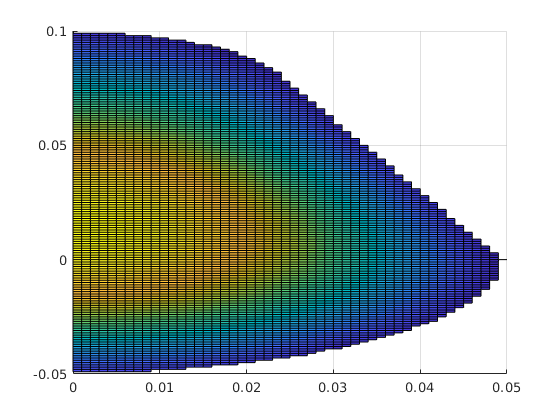
\includegraphics[width = 1\textwidth]{Disorder_inducing_pear_CO2_boven.png}
\caption{CO2 voor Disorder inducing.}
\end{figure}
\end{column}
	
\begin{column}{0.48\textwidth}
\begin{figure}
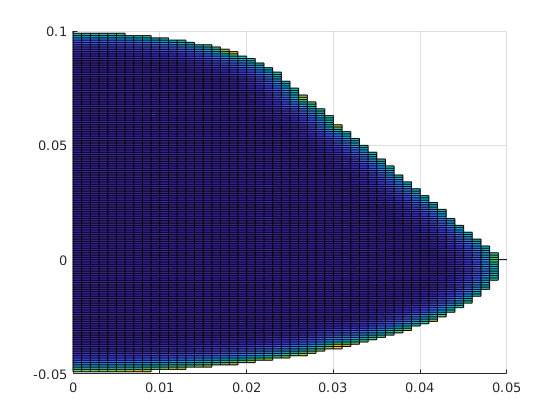
\includegraphics[width = 1\textwidth]{Disorder_inducing_pear_O2_boven.png}
\caption{O2 voor Disorder inducing.}
\end{figure}
\end{column}
\end{columns}
	
\end{frame}

\begin{frame}
\frametitle{Resultaten: Precooling}
\begin{columns}
\begin{column}{0.48\textwidth}
\begin{figure}
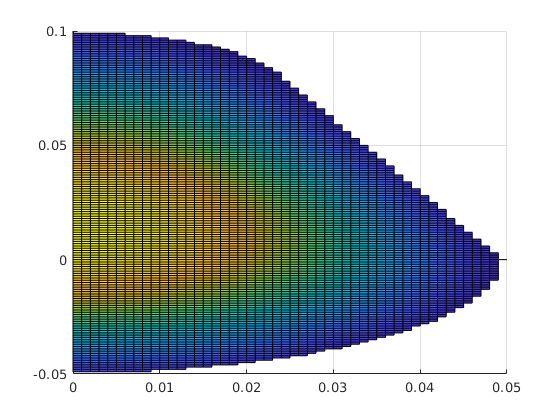
\includegraphics[width = 1\textwidth]{Precooling_pear_CO2_boven.png}
\caption{CO2 voor Precooling.}
\end{figure}
\end{column}
	
\begin{column}{0.48\textwidth}
\begin{figure}
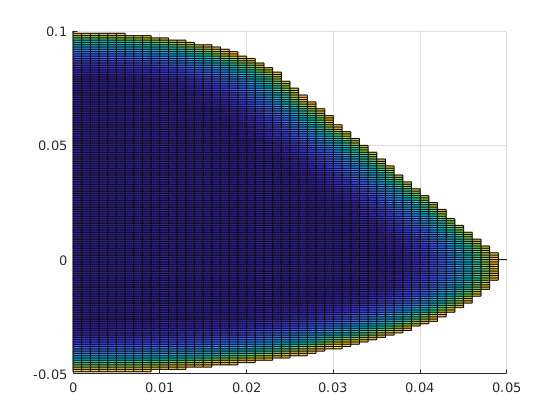
\includegraphics[width = 1\textwidth]{Precooling_pear_O2_boven.png}
\caption{O2 voor Precooling.}
\end{figure}
\end{column}
\end{columns}
\end{frame}

\begin{frame}
\frametitle{Resultaten: Refrigerator}
\begin{columns}
\begin{column}{0.48\textwidth}
\begin{figure}
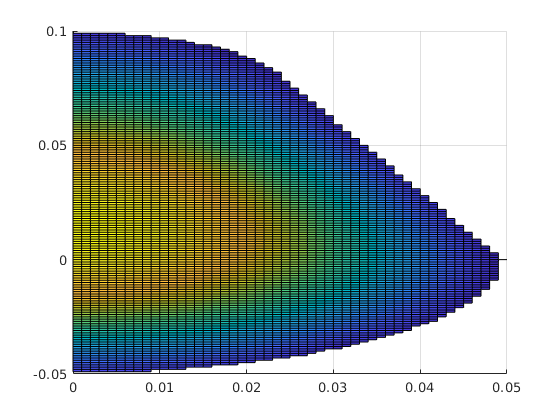
\includegraphics[width = 1\textwidth]{Refrigerator_pear_CO2_boven.png}
\caption{CO2 voor Refrigerator.}
\end{figure}
\end{column}
	
\begin{column}{0.48\textwidth}
\begin{figure}
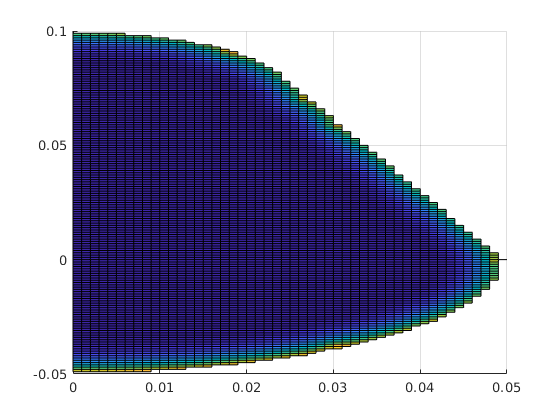
\includegraphics[width = 1\textwidth]{Refrigerator_pear_O2_boven.png}
\caption{O2 voor Refrigerator.}
\end{figure}
\end{column}
\end{columns}
\end{frame}

\begin{frame}
\frametitle{Analytische oplossing O2}
$r^2*C_u'' +2*r*C_u' - B^2*r^2*C_u = 0$ \\ $ \Leftrightarrow C_u(r) = C_1*\frac{exp(-B*r)}{r}+C_2*\frac{exp(B*r)}{B*r}$. Die voldoen aan randvoorwaarden: $C_u'(0) = 0$ en $ C_u'(R) = \frac{h_u}{Dur}*(C_u-C_{uamb})$.\\
Dit geeft de oplossing:\\
$ C_u(r)= \frac{R^2*h_u*C_{uamb}*sinh(B*r)}{r*(Dur*cosh(B*R)*B*R-Dur*sinh(B*R)+R*h_u*sinh(B*R))}$
\end{frame}

\begin{frame}
\frametitle{Vergelijk analytische en numerieke oplossing voor cirkel}
\begin{columns}
\begin{column}{0.48\textwidth}
\begin{figure}
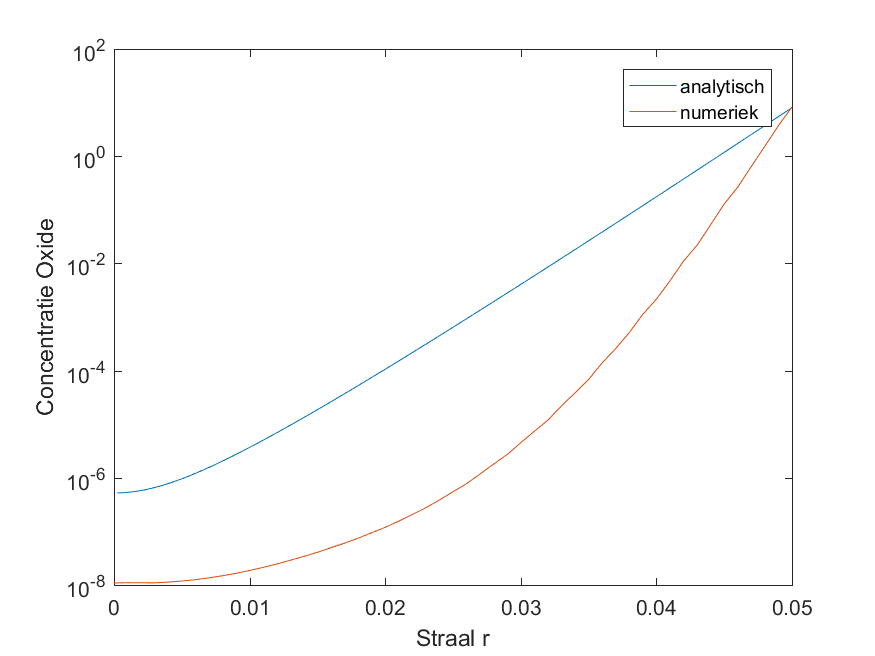
\includegraphics[width = 1\textwidth]{Precooling_sphere_O2_analytical.png}
\caption{Vergelijk analytische en numerieke oplossing van O2 voor de Precooling.}
\end{figure}
\end{column}
	
\begin{column}{0.48\textwidth}
\begin{figure}
\includegraphics[width = 1\textwidth]{Precooling_sphere_O2_analytical_finemesh.png}
\caption{Vergelijk analytische en numerieke oplossing van O2 voor de Precooling voor een fijner mesh.}
\end{figure}
\end{column}
\end{columns}
\end{frame}

\begin{frame}
\frametitle{Vergelijk analytische en numerieke oplossing voor cirkel}
\begin{columns}
\begin{column}{0.48\textwidth}
\begin{figure}
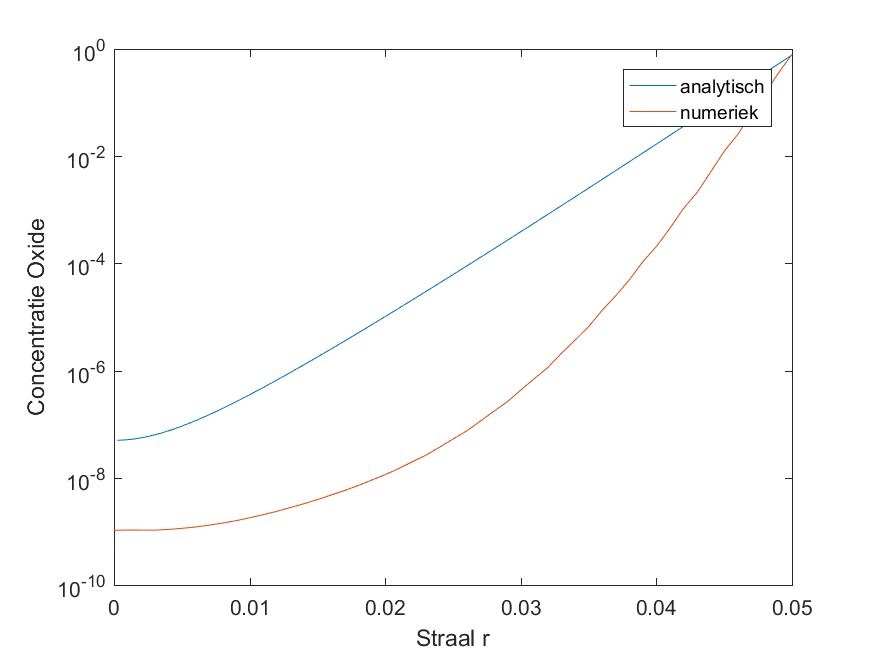
\includegraphics[width = 1\textwidth]{Optimal_CA_sphere_O2_analytical.png}
\caption{Vergelijk analytische en numerieke oplossing van O2 voor de Optimal CA.}
\end{figure}
\end{column}


\begin{column}{0.48\textwidth}
\begin{figure}
\includegraphics[width = 1\textwidth]{Optimal_CA_sphere_O2_analytical_finemesh.png}
\caption{Vergelijk analytische en numerieke oplossing van O2 voor de Optimal CA voor een fijner mesh.}
\end{figure}
\end{column}
\end{columns}
\end{frame}



\begin{frame}
\frametitle{Verloren tijd, onverwachte resultaten en mogelijke verbeteringen}
\begin{itemize}
\item Lang gedacht dat de niet lineaire oplossing in matlab fout was. (Terwijl correct)
\item Mogelijke verbeteringen
\begin{itemize}
\item Gebruik maken van het sparse zijn
\item Multigrid methode proberen
\item Zoeken naar een betere preconditioner
\item Opkuisen van cpp file
\item mesh in cpp zelf laten maken (en matlab volledig uitschakelen)
\item ...
\end{itemize}
\end{itemize}
\end{frame}

\end{document}